\subsection{Osmotic Scheduling in Dynamic Systems}
% 3+ pages (complicated setup, no?)
In this last experiment we test the behaviour of our osmotic scaling and scheduling method in a dynamic system.
Since dynamic changes of the system make-up are a core part of edge computing, and our approach is explicitly constructed with these dynamic factors in mind, we believe it is important to test the efficacy of our approach in such a scenario.
Because a lot of components have already been analyzed in-depth, and results are most clear when only one factor is tested at any given time, we choose to use the request origin as the dynamic  system component.
With the experiment we test how our proposed approach handles requests originating from different regions of the overall system over time.
\subsubsection{Setup}
For this experiment we once again use the globally distributed scenario as our network topology, and apply a constant request rate of 25\gls{rps}.
Each of the three cities present in the topology additionally has a probability function associated with it, which determines the chance of a request originating from that city.
These probability functions for the cities are set up in such a way that most of the requests originate from only one of the cities for a given time period.
After some time the active city changes and the requests gradually start to come from another city.
The periods and changes are set up in such a way that over the course of the 2000 second long simulation each of the cities is the main originator of requests at one point.

\subsubsection{Results}

\begin{figure}
    \centering
    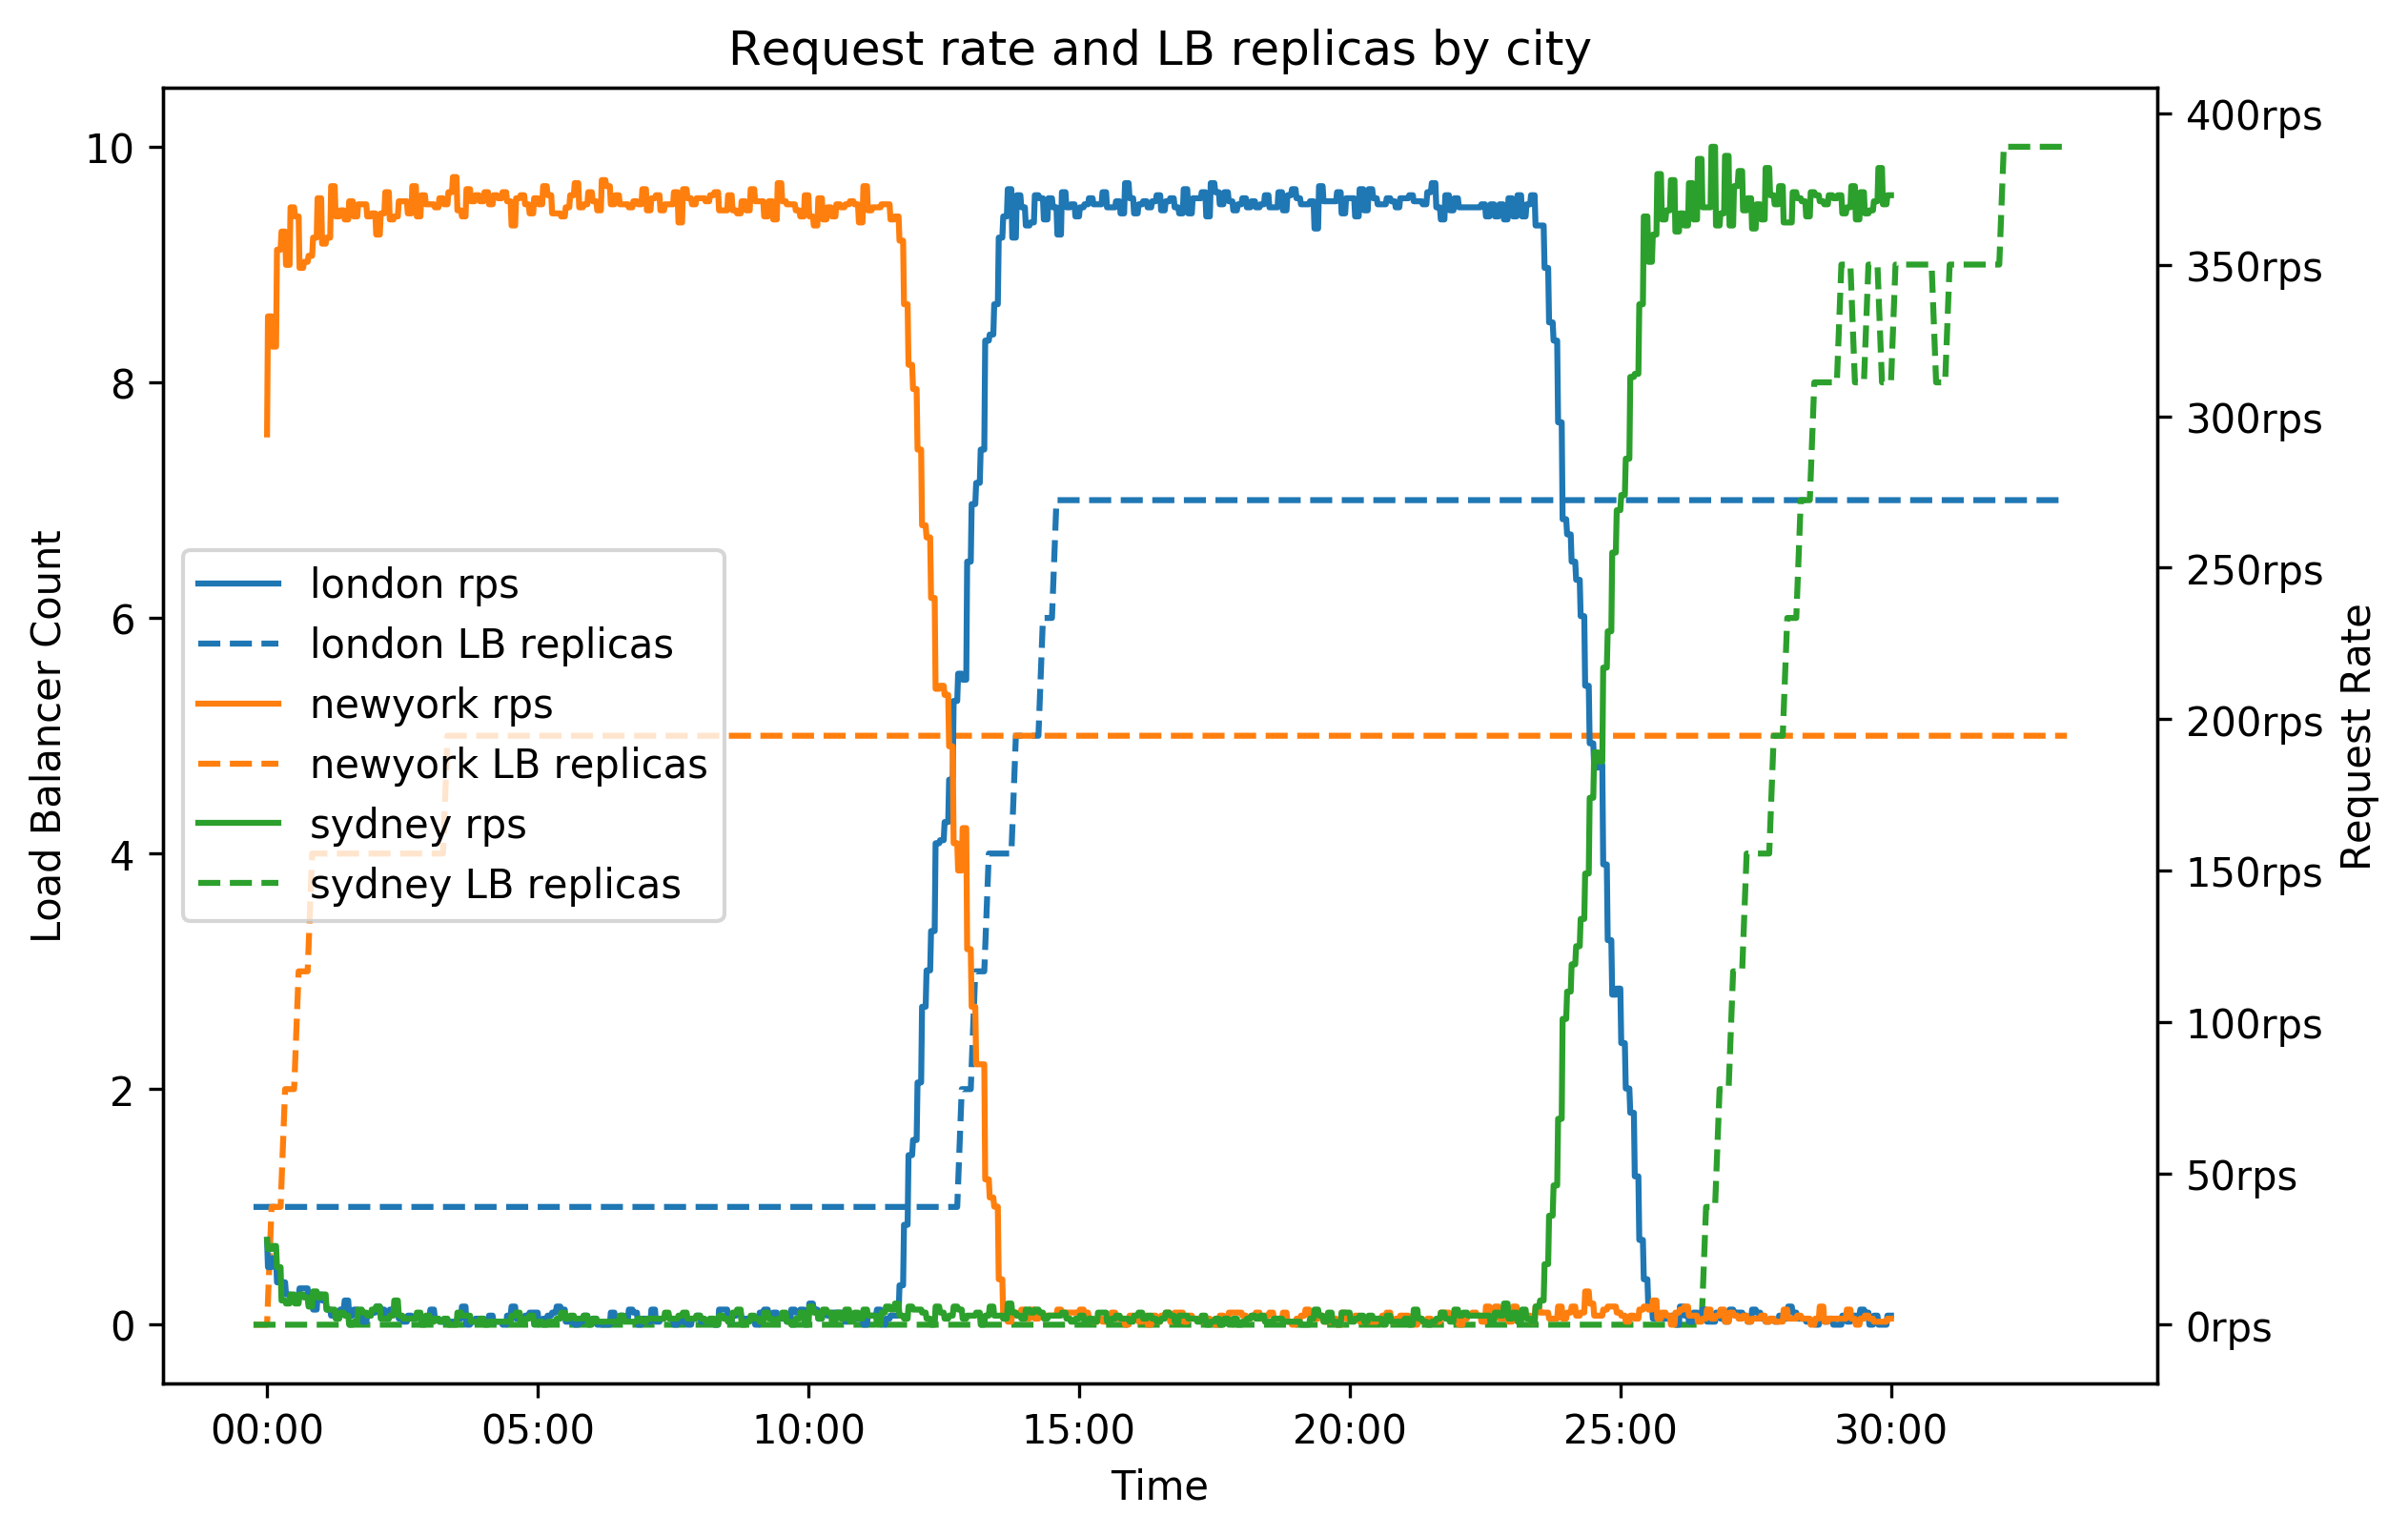
\includegraphics[width=14cm]{graphics/graphs/osmotic_dynamic_region_rps_lb_relicas_corrected.png}
    \caption{Load balancer replica count per city over changing request origins}
    \label{fig:osmotic_dynamic_lb_replicas}
\end{figure}

\begin{figure}
    \centering
    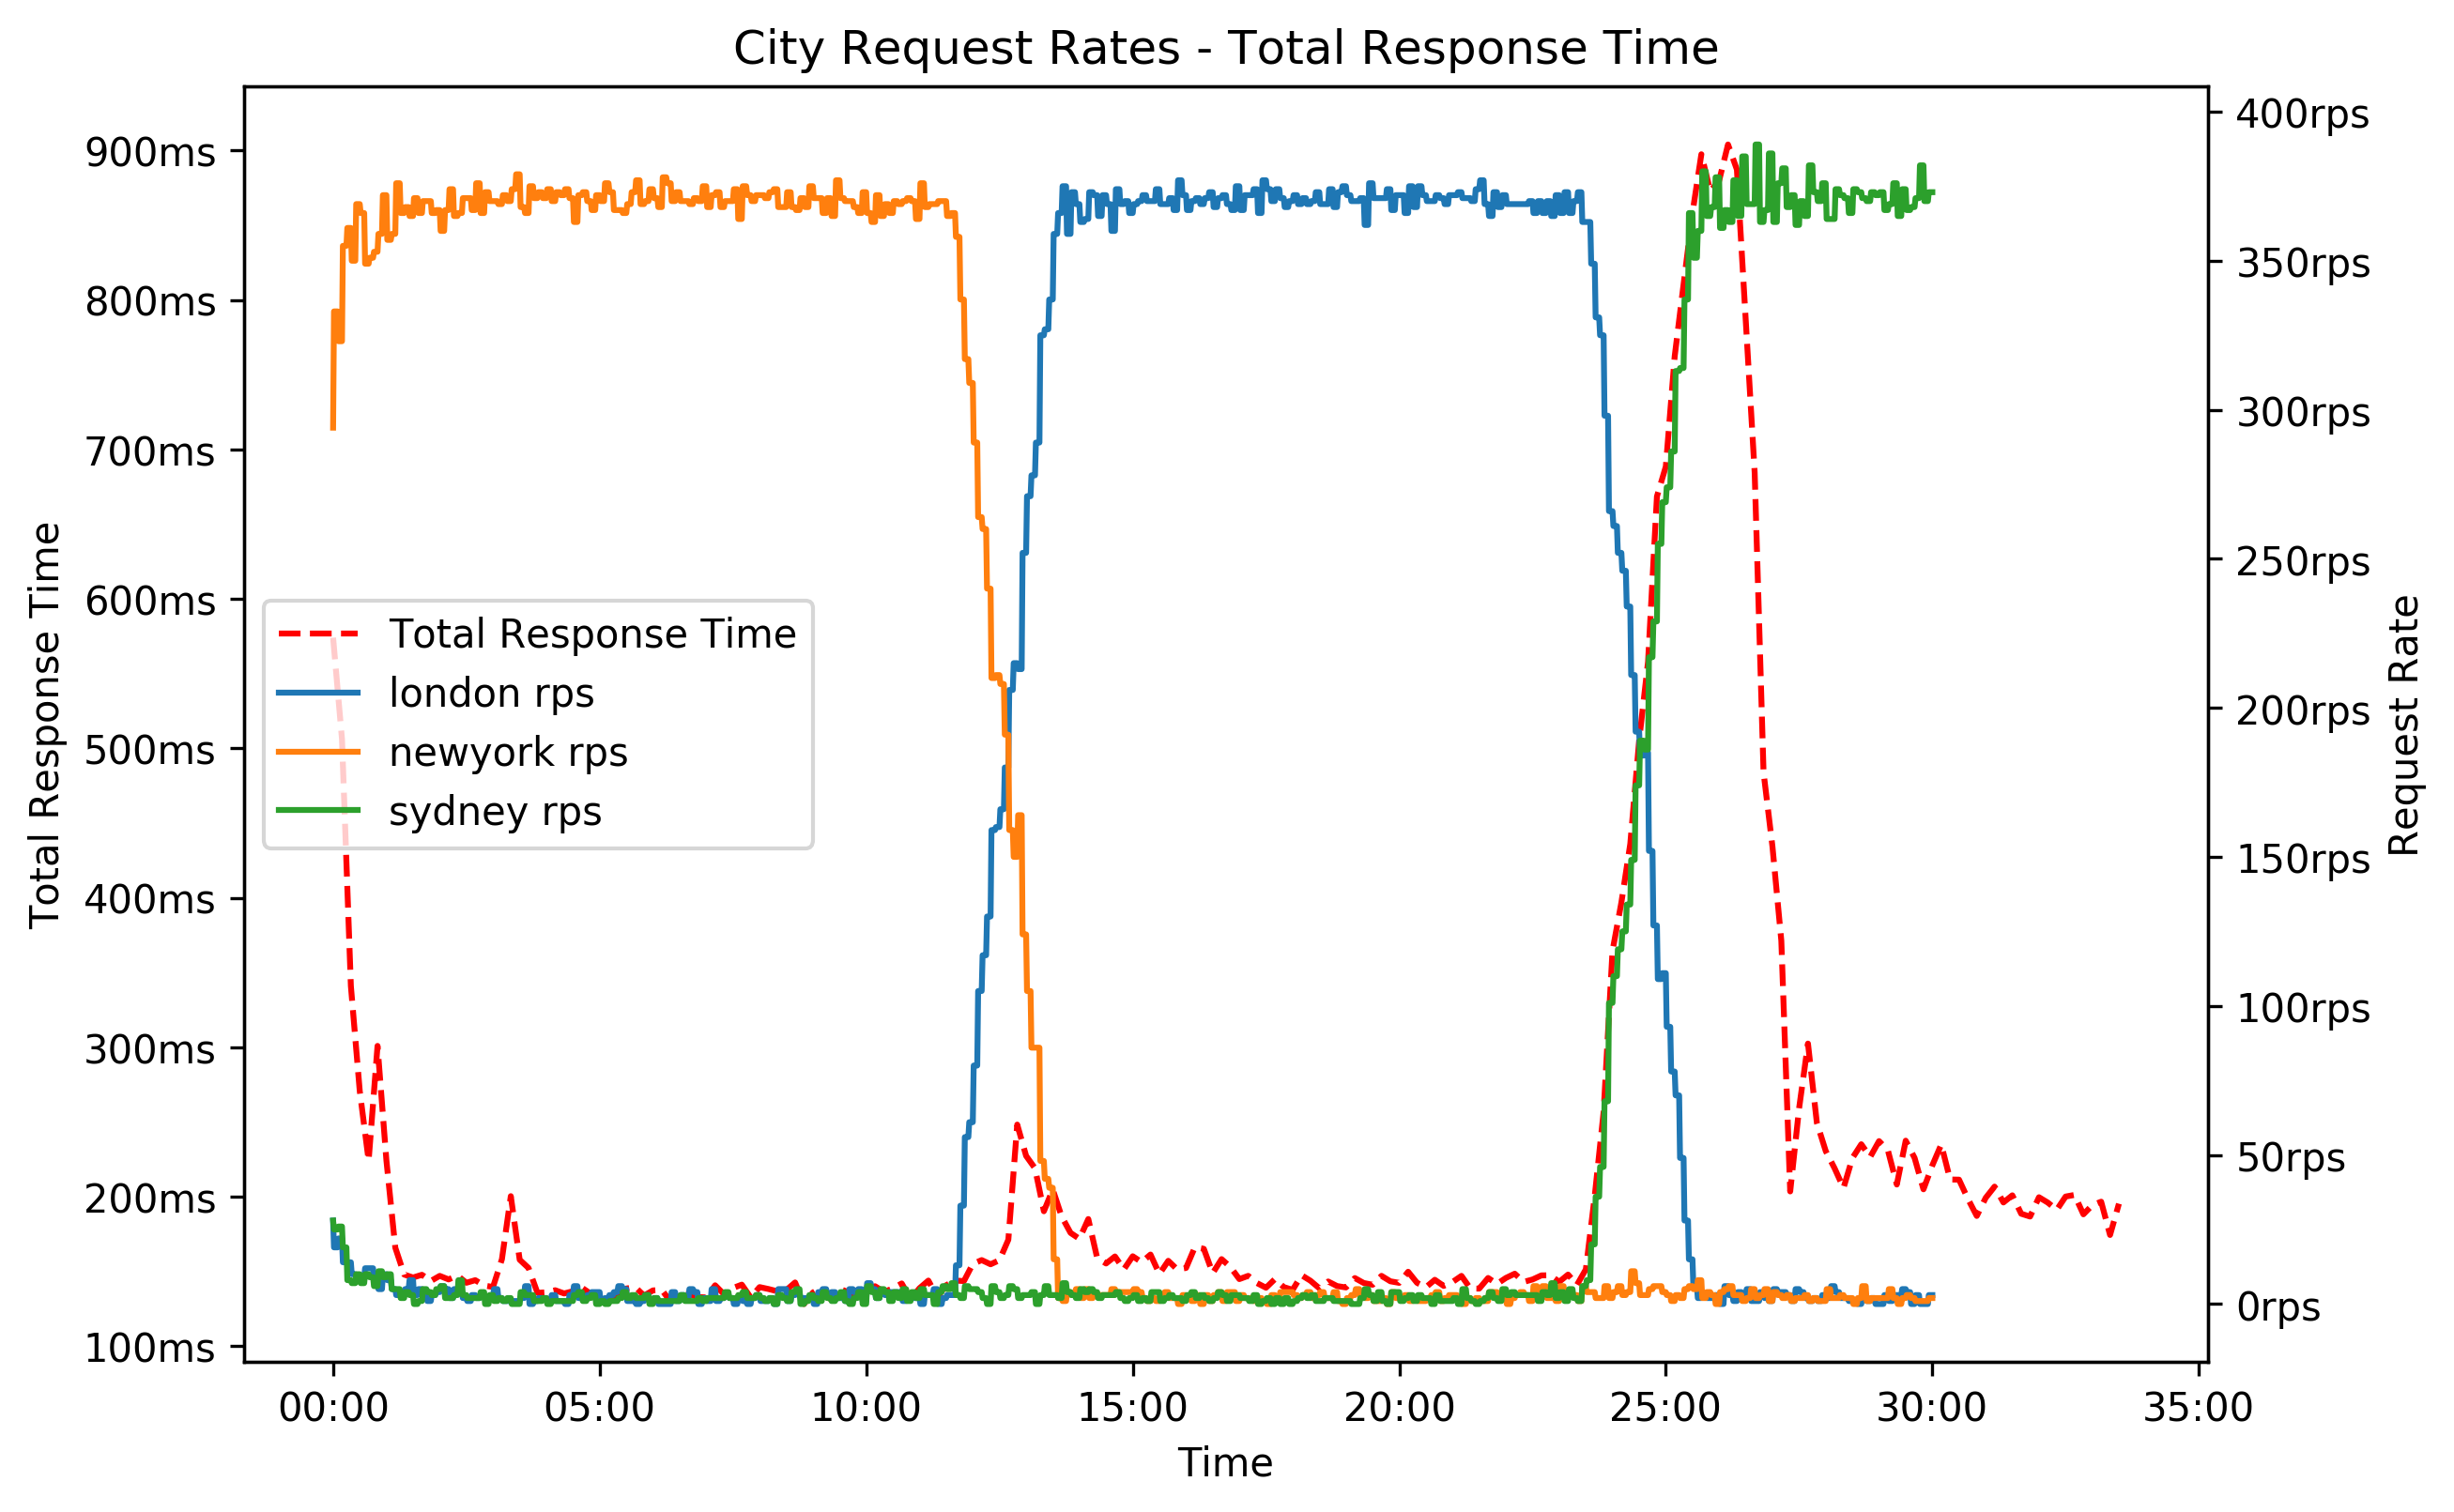
\includegraphics[width=14cm]{graphics/graphs/osmotic_dynamc_region_rps_trt_corrected.png}
    \caption{Total response time over changing request origins}
    \label{fig:osmotic_dynamic_trt}
\end{figure}

\begin{figure}
    \centering
    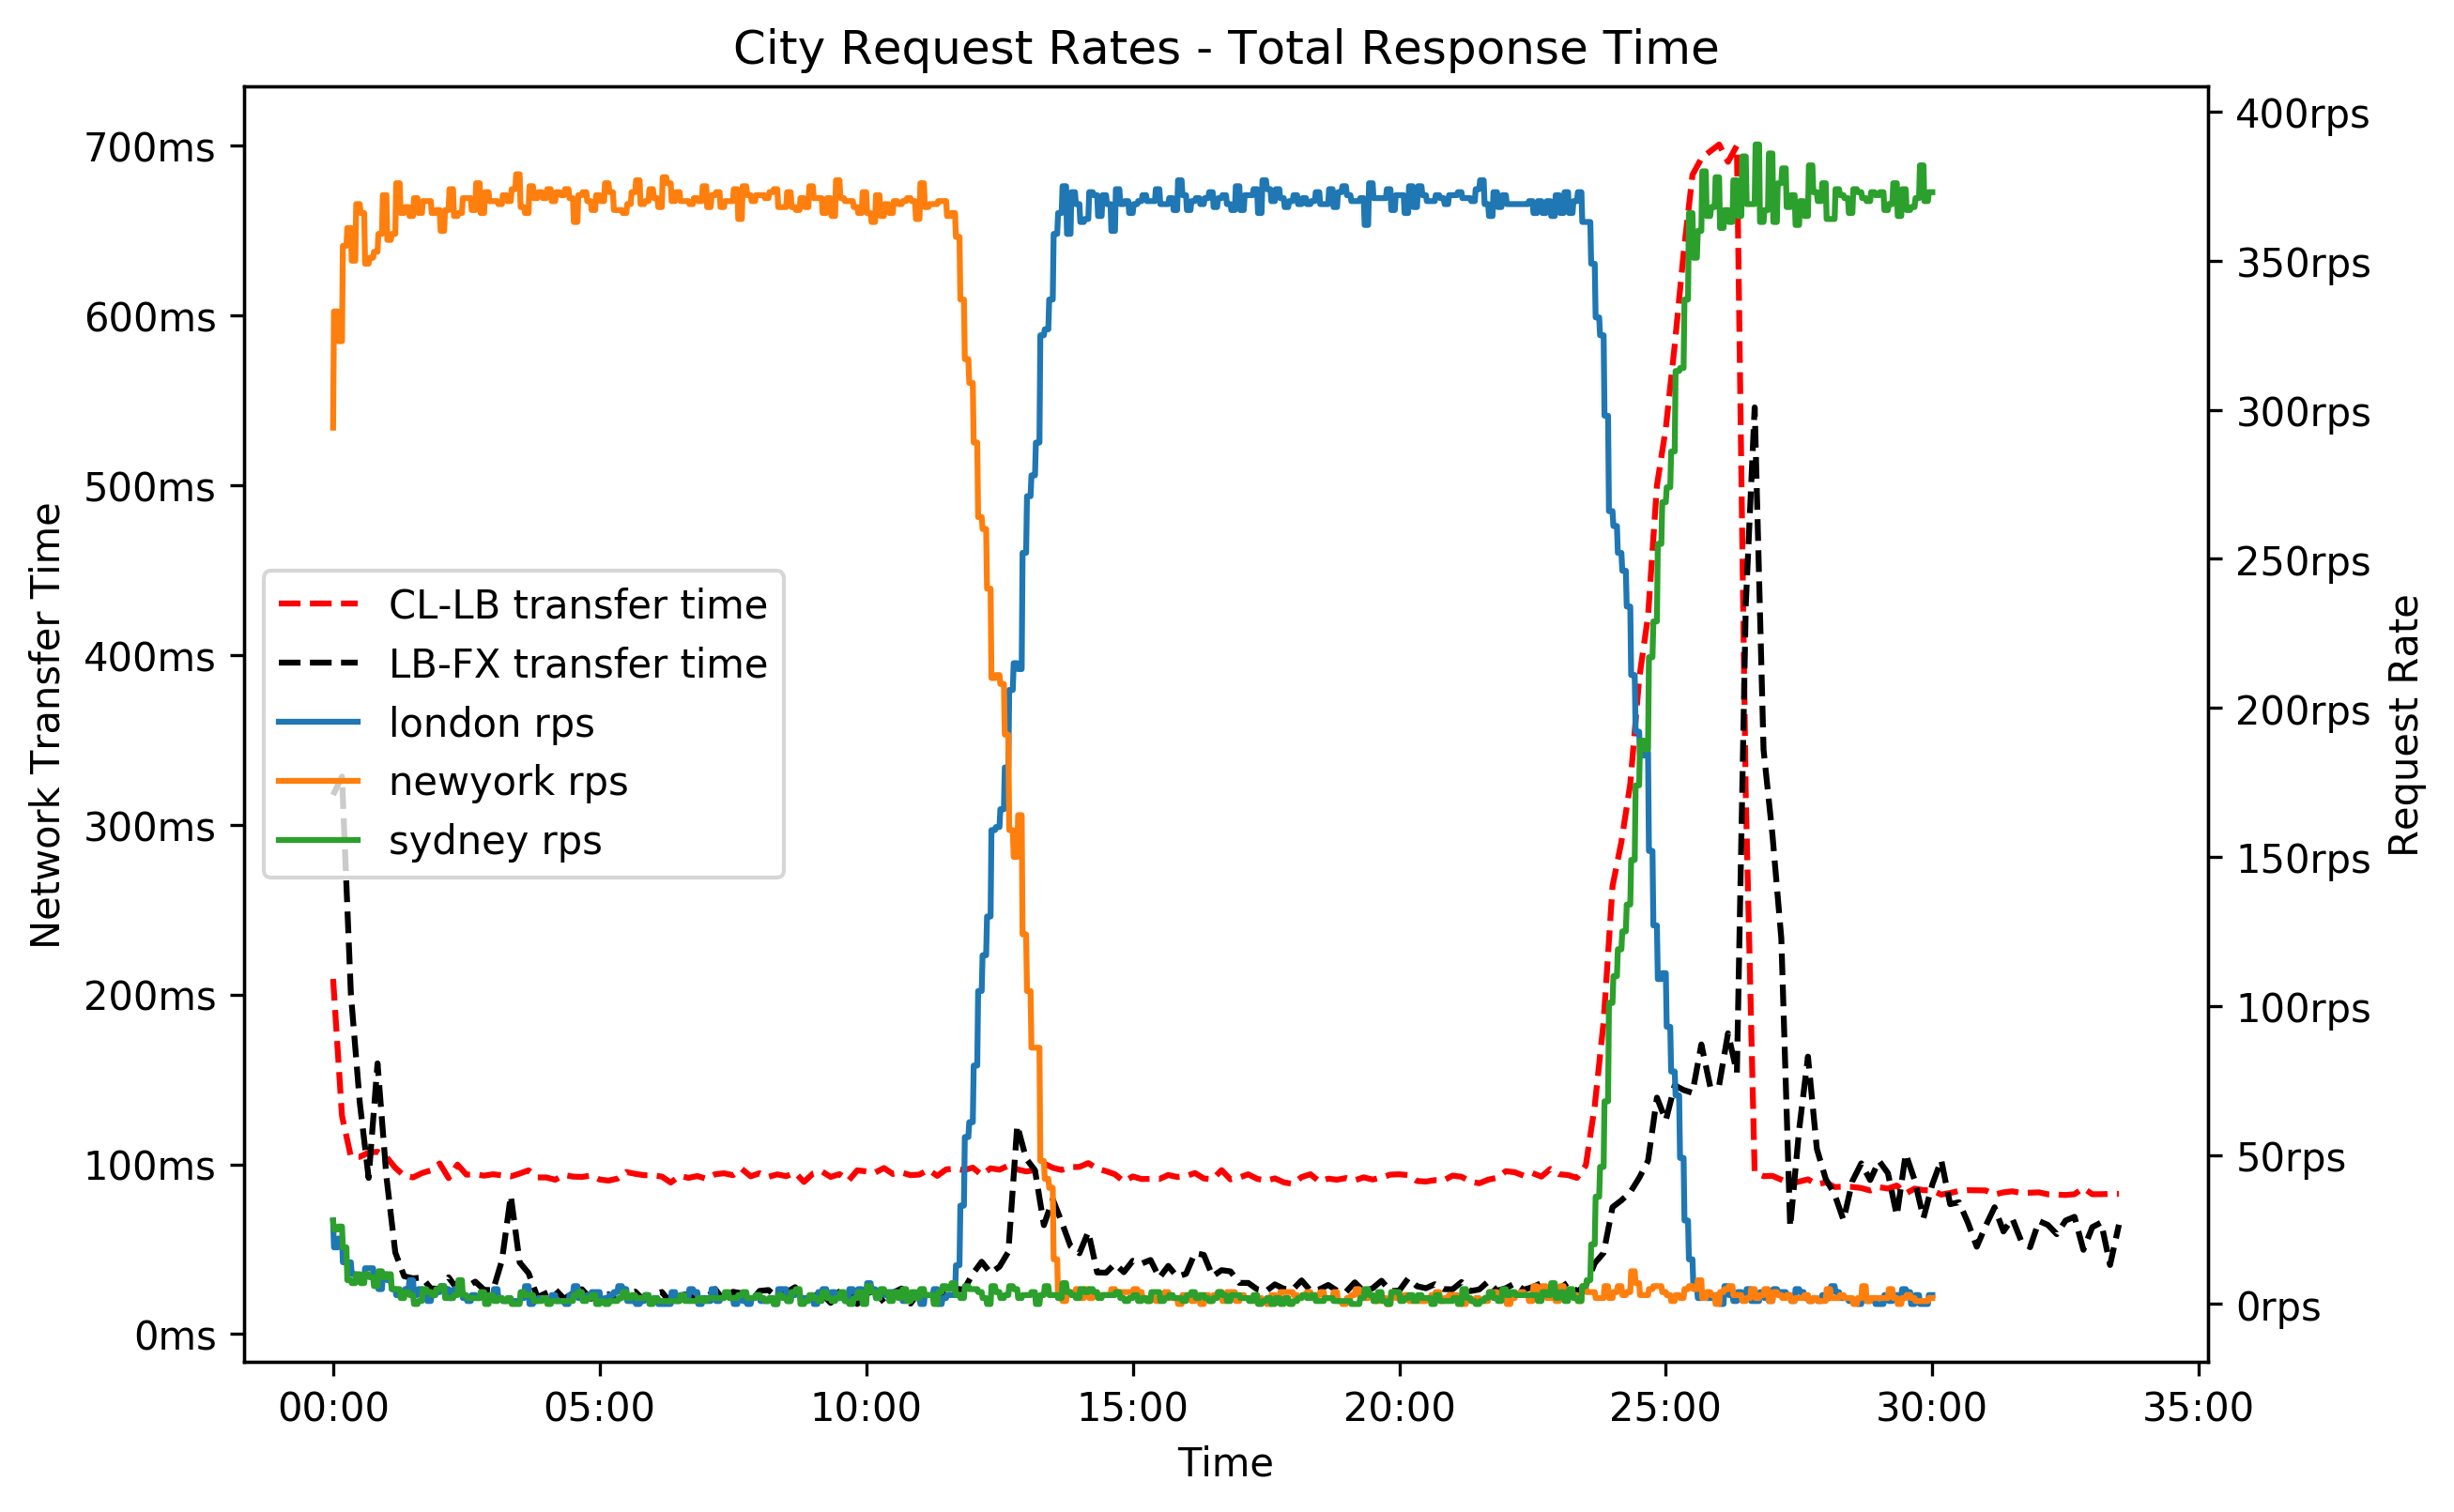
\includegraphics[width=14cm]{graphics/graphs/osmotic_dynamic_region_tx_times_corrected.png}
    \caption{Client to load balancer, and load balancer to function transfer times over changing request origins}
    \label{fig:osmotic_dynamic_tx}
\end{figure}

First of all, the results show that the osmotic scaling and scheduling component does indeed take the request origin into account when deciding on the number and location of new load balancer replicas.
Figure \ref{fig:osmotic_dynamic_lb_replicas} shows this in action.
While originally load balancers are only spawned in one city, because all requests originate from it, once requests start coming from another city, another load balancer instance is deployed in that city, as can be seen around timestamps 00:12 and 00:25 in Figure \ref{fig:osmotic_dynamic_lb_replicas}.

The effect this has on the system at large can also be observed easily, as Figure \ref{fig:osmotic_dynamic_trt} shows.
Here we can see that while the total response time of the system spikes once requests start to originate from another city, it starts to stabilize and come down to previous levels again once load balancers are present in the new city.
Please note that the \gls{trt} values shown in Figure \ref{fig:osmotic_dynamic_trt} are a moving average over a 10 second window, since this removes noise from the plot, making it more readable.
Likewise the request rate per city in Figures \ref{fig:osmotic_dynamic_lb_replicas}, \ref{fig:osmotic_dynamic_trt}, and \ref{fig:osmotic_dynamic_tx} is a moving average over a 5 second window, and displays the request rate for all functions deployed in the system.

Just like with the \gls{trt}, Figure \ref{fig:osmotic_dynamic_tx} shows that the request transfer time between client and load balancer, as well as between load balancer and function replica also spike when traffic originates from a different city.
There too, though we see that it returns to previous levels once load balancer replicas become available near the request origin.
